\chapter{Caractérisation de la navigabilité d'une tentacule}
\begin{figure}[!ht]
    \centering
    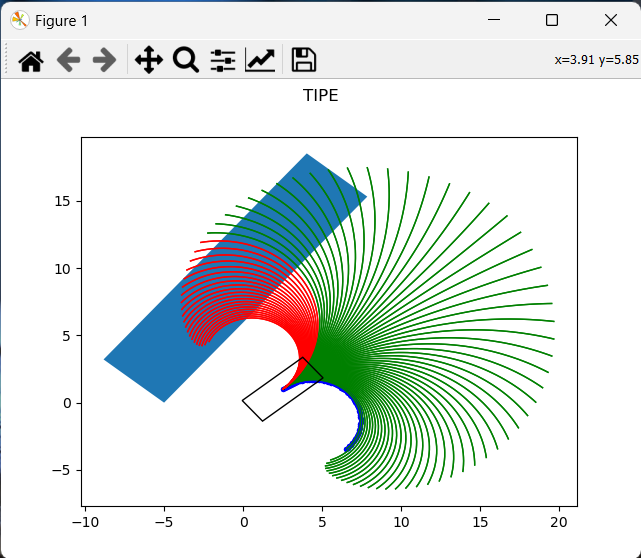
\includegraphics[scale=0.7]{collision.png}
\end{figure}
\vspace{120pt}

\begin{mintedbox}{python}
"""
Trace les tentacules en différentes couleurs, à l'arrêt, selon qu'elles soient navigables ou non.
"""
class Tentacule:
    """
    Objet tentacule, dépendant d'une voiture, et déterminé par son ordre et son angle de braquage.
    """
    def get_zone_support(self):
        if self.voiture.vitesse < 3:
            self.dist_zone_support = 1.4 + 0.2*self.voiture.vitesse/3  # formule empirique p.123 eq(9.6) thèse
        elif 3 <= self.voiture.vitesse <= 15:
            self.dist_zone_support = 1.6 + 0.6 * (self.voiture.vitesse-3) / 15  # idem
        else:
            raise ValueError("La vitesse est trop élevée !")
        self.zone_support = shapely.geometry.LineString( self.get_parametric()).buffer(self.dist_zone_support)
        return self.zone_support

    def is_navigable(self, objets_alentours):
        self.zone_to_be_clean = self.get_zone_support().intersection(self.voiture.get_espace_collision())
        for objet in objets_alentours:
            if objet == self.voiture:  # Pas grave si la tentacule cogne sa propre voiture
                pass
            elif self.zone_to_be_clean.intersection(objet.shapely_poly).is_empty is False:
                self.patch.set_color("red")
                return False
        return True


class Voiture:
    """
    Objet voiture, défini par sa forme. D'autres paramètres fixes sont définis après, on pourra les mettre en paramètre plus tard si plusieurs voitures il y a.
    """
    def get_espace_collision(self):
        self.distance_collision = self.vitesse**2 / 2*self.accel_lat_max
        self.espace_collision = shapely.geometry.Point((self.x, self.y)).buffer(self.distance_collision + self.longueur/2)
        return self.espace_collision

    def is_tentacule_navigable(self, tentacule, objets_alentours):
        return tentacule.is_navigable(objets_alentours)

    def choix_tentacule(self, tentacules_navigables):
        try:
            # On prend la 1ere tentacule lisse qu'on trouve
            for tentacule in tentacules_navigables:
                if tentacule.lisse is True:
                    return tentacule
            # Si aucune n'est lisse, on prend la 1ère
            return tentacules_navigables[0]
        except IndexError:
            raise "AUCUNE TENTACULE NAVIGABLE"

    def get_tentacules_navigables(self, objets_alentours):
        tentacules_navigables = []
        for tentacule in self.tentacules:
            if tentacule.is_navigable(objets_alentours):
                tentacules_navigables.append(tentacule)
        return tentacules_navigables

    def _simu(self, simu):
        self.simu = simu


class Obstacle():
    def __init__(self, patch):
        self.patch = patch
        self.x, self.y = self.patch.get_center()
        self.shapely_poly = shapely.geometry.Polygon(
            (self.patch.get_transform()).transform_path(self.patch.get_path()).vertices)


class Obstacle_fixe(Obstacle):
    def __init__(self, patch):
        super().__init__(patch)

\end{mintedbox}
